%
% verschmierung.tex
%
% (c) 2020 Prof Dr Andreas Müller, Hochschule Rapperswil
%
\begin{frame}
\frametitle{Verschmierung}
\begin{definition}
{\em Verschmierung} ist
Genauigkeitsverlust durch grosse Zwischenresultate
\end{definition}

\begin{block}{Beispiel}
Berechnung von $e^{-a}$ mit Hilfe der Taylorreihe
\[
e^x = 1 + x + \frac{x^2}{2!} + \frac{x^3}{3!} + \frac{x^4}{4!} +\dots
=
\sum_{k=0}^\infty \frac{x^k}{k!}
\]
\end{block}

\begin{center}
\begin{tabular}{|l|>{$}r<{$}|}
\hline
Datentyp            & e^{-30} \\
\hline
\texttt{float}      & -7.2959523438\cdot 10^{\phantom{-}4\phantom{0}}\\
\texttt{double}     &  6.1030424789\cdot 10^{-6\phantom{0}}\\
\texttt{long double}& -1.2489259417\cdot 10^{-8\phantom{0}}\\
\hline
exakt               &  9.3576229688\cdot 10^{-14}\\
\hline
\end{tabular}
\end{center}

\end{frame}

\begin{frame}
\frametitle{Zwischenresultate}
\ifthenelse{\boolean{presentation}}{
\vspace{-22pt}
}{}
\begin{center}
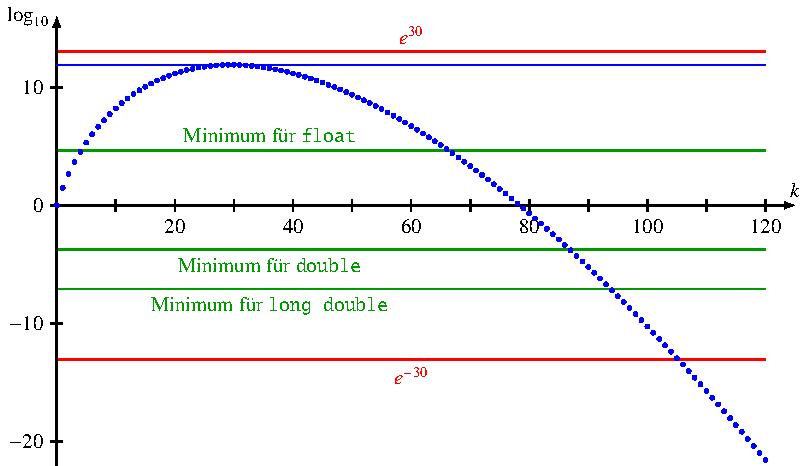
\includegraphics{../../buch/chapters/10-arithmetik/figures/verschmierung.pdf}
\end{center}
\end{frame}
